% ------------------------------------------------------------------------------
% Chapter 1
% Delete this content and replace with your own
% ------------------------------------------------------------------------------
\chapter{Technique Taxonomy} % enter the name of the chapter here


\section{Challenges}
\subsection{Problem Challenges}
The key challenges posed by our problem statement revolve around having a method for efficiently updating of dashboards without re-querying the entire database. We also need to alert the widgets about the update after each dashboard refresh and display the data. The data is streamed in real time so such updates need to minimally be faster than the input rate to prevent queuing. Otherwise the system may suffer from cascading failures due to rate overflow and lack realtime-ness.

\subsection{Literature Survey}
Our first key challenge is to identify the existing state of the art techniques and work done in the above mentioned fields. This involves benchmarking databases and selecting one which best suits our use-case. We used YCSB\cite{YCSB} and tested different databases on a variety of workloads. This paper gives performance benchmarks for various databases on simulated workloads. It also gives an interface to extend for newer databases and gives us the option to test them on custom workloads. This makes it a standard when doing database benchmarking. Since, our use case is read-heavy, we primarily focused on database query performance.

We also studied survey papers for indexing\cite{Indexing}, query processing\cite{QueryProcessing}, caching\cite{Caching}, and data visualization\cite{VisualizationTechniques} to understand existing literature and techniques. The papers cover important literature in the field and help further group the topics into sub-fields. The papers provide a general idea of the existing work and the future research direction in these fields.

\subsection{Finding Novel Ideas}
We did not want to solely replicate  existing state of the art ideas. We also wanted contribute a novel idea of our own. This is one of the most challenging aspects of the project since developing and testing novel ideas require a lot of thought and experiments to confirm our intuition. We broadly identified two fields, namely query processing and caching to implement new ideas. We used the DbToaster\cite{DbToaster} and FlashStore\cite{FlashStore} paper as our primary reference. The papers match our use-case and provide significant performance improvement on the base model.

\subsection{Integrating Sub-systems}
It is important to integrate the various subsystems without sacrificing performance. The benefits of indexing, caching and fast query processing should all be complementary to the overall goal of the project. We need to ensure the access patterns of our in-memory caching is in line with the database accesses and that we index on the appropriate columns. Our queries then need to take advantage of our indexes cache. Without complimentary subsystems, the benefits of each sub-domain may not be fully realized. Hence, is is an important engineering challenge.

\subsection{Technical Challenges}
We also faced minor technical challenges to ensure a common environment for all our team members. With each one of us using a different operating systems(eg: Debian Linux, Mac and Windows), it was important for us to address this problem early. We used Docker\cite{Docker} to this purpose. Since none of us have had experience with advanced database techniques, there was a significant learning curve.

\section{Technique Taxonomy}
The following section contains the techniques we used for addressing the challenges posed.

\subsection{Indexing}
An interactive dashboard is measured by the performance of indexing and query processing techniques under the hood. For indexing, we explored in-house techniques offered by MySQL\cite{MySQL}. MySQL indexing scheme for both primary and secondary indexes work quite well for our use-case and we did not feel the need to develop something to replace this. We also evaluated other databases but for read heavy queries MySQL offered the best performance. 

We evaluated other indexing techniques like Learned Indexing\cite{LearnedIndexing} which uses machine learning to reduce the search space of possibilities and find the appropriate index. Learning techniques help prune through the search space and assign each data point in this space with a cost using the cost model. The optimization strategy is then responsible for choosing the best data point that can represent the best index. In a way, it uses heuristics without needing any domain knowledge. The domain knowledge in this case is presented by the training set. The following image shows the interaction between the various components in the learning model.
\begin{center}
    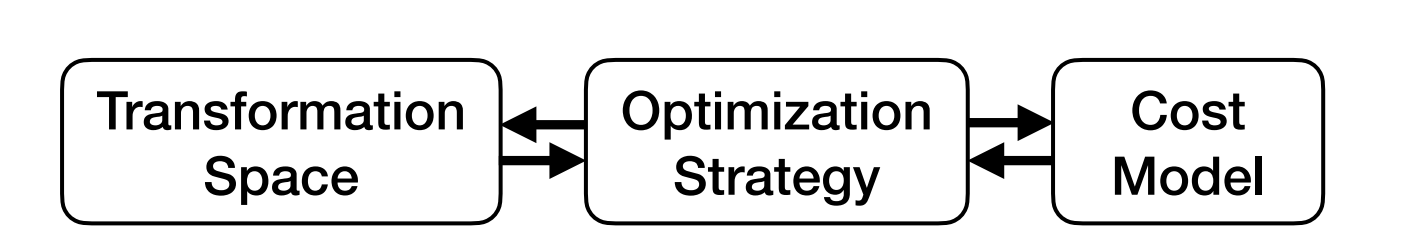
\includegraphics[scale=0.25]{ML.png}
\end{center}

We also explored Adaptive Data Series Indexing\cite{ADS}, which uses a strategic style of indexing to reduce the data-to-query gap. Instead of building the complete index over the complete data up-front and querying only later, we interactively and adaptively build the parts of the index tree necessary for the query. Although the approach beats the state-of-the-art indexing techniques, it is unsuitable for our target scenario. We query across the entire database, not a specific subsection, and thus adaptive indexing provide little to no tangible benefits. We decided to stick with MySQL indexing techniques and focus on other areas for performance.

Inverted indexing technique\cite{InvertedIndexing} and other techniques presented in the paper by Lehman et al.\cite{MainMemoryIndexStructures} largely covered indexing structures for main memory databases. These group of ideas are borrowed from the field of information retrieval and improve performance when we look to perform operations which retrieve specific information from a text document. However, these techniques are relatively complex and have pre-existing hardware requirements. When compared to MySQL in-house indexing techniques, the performance benefits are not significant enough to justify investment.

\subsection{Delta Queries}
Many existing works build upon the concept of incremental view maintenance. In incremental view maintenance, materialized views compute and apply incremental changes to stay up to date instead of recomputing the contents from the base relation. We focused heavily on delta queries\cite{IncrementalMaintenance}, a technique to compute the incremental change and in turn ensure efficient dashboard updates. Griffin et al.\cite{IVMWithDuplicates} explains the base idea behind delta queries.

We used DbToaster\cite{DbToaster} and the follow up paper\cite{DbToaster2} as the primary reference for the part of the problem. The papers propose high performance query executors which parse original queries into a query that hits a minimal set of tuples in the database. These are then used to update in-memory views which help supply the result of the original query. In terms of target applications, it aims to help high volume data streams that have frequent updates and need fast and low latency read queries. Performance is also improved by doing computation in main memory. In our case, each dashboard query is transformed into a smaller query which only queries against a smaller subset of pre-computed results. The idea reduces the search space of the query, thereby resulting in a quicker response time.

The ideas of change data capture and delta queries for the purposes of incremental view maintenance have been adopted by other existing works such as CoNoSQLDBs\cite{DeltaNoSQL}\cite{CDC-CoNoSQL}, object-oriented databases\cite{ObjectOriented-IVM} and in data warehouse environment\cite{IVM-Algorithm}. This gives us the confidence to apply delta queries to solve one area of our problem. In the rest of the report, we explore additional areas where we can extract faster query results.

We also looked at incremental deferred view maintenance\cite{IDeferredVM}. The paper introduces the concept of auxiliary tables and how they are maintained in memory to support deferred refreshes of data interface. The key takeaway is how the auxiliary tables support delta query processing in-memory. Since we aim to support dashboard interactivity, we allow users to update database in multiple different manners. For multiple insertions, we look to He et al.\cite{BatchIVM}.

A similar paper that we explored is in-situ query processing ideas presented by Olma et al.\cite{InSitu}. The core idea here is about query processing using a combination of data partitioning and indexing techniques. The in-situ query engine proposed in this paper builds indexes on the fly for different partitions of data. The idea is a little overkill for our specific use case, especially due to the lack of sharding. However, the paper facilitated further exploration of in-situ techniques, eventually leading to caching techniques.

\subsection{In memory caching}
We store auxiliary tables which contain data for the aggregate widgets on the dashboard. It is thus important to explore techniques which enable us to cache the data for further access performance. Zhou et al.\cite{LazyViews} argue for lazy persistent updates on the views and caching the data in-memory. It uses a way to combine writes from several transactions, which are pushed onto the main database only when a read query is made on the one of the tuples updated in the write queries. While it works well in practice for read-write queries, it is not as relevant in our scenario as multiple reads occur immediately after a write.

Since we are storing a minimal set of key-value pairs in our auxiliary tables, we can migrate it to caches inside memory. We explored the FlashStore\cite{FlashStore}\cite{FalshKVStore}, BloomStore - an optimization on FlashStore\cite{BloomStore} Memc3\cite{Memcached} paper in this regard, all of which focus on caching models. Our eventual implementation is derived from the FlashStore\cite{FlashStore} paper. FlashStore exploits the methods of building an in-memory caching model using a custom hash table. The caching model proposed is persistent and is built to handle a high throughput. The hashing scheme proposed is also built to handle concurrency using a key-wise locking scheme. 

In terms of the higher level model, it is a write-back cache. Data is written onto the cache and transferred to the database only when cache line is evicted. The model works best for read heavy workloads. Another option is a write-around cache, which provides good write performance but has a slower read performance as every new read is a cache miss. It is completely the opposite of our target scenario. The last option is write-through cache, which ensures consistency and is tolerant to failures. However, each operation being performed twice thus slowing down performance. Therefore, we designed our cache with many of the techniques from FlashStore in mind.

For the purpose of scaling our model for larger workloads, we also explored distributed caching models\cite{DistibutedCaching}. Such models help mitigate the issue of limited caching memory. Such models are useful when the size of the data exceeds the hardware limits on a single phycial machine. In such cases, the cache itself is distributed across machines with the data mapped onto it. This idea forms the core of data sharding. We also explored modern databases such as Oracle\cite{Oracle} to compare how these techniques are implemented. The paper explains an end-to-end implementation of a database which uses indexing, sharding, query processing and execution. This was important to read as it helped us validate some of our intuitions.

\subsection{Data Interface}
The direct representation of relations on screen is significantly easier to navigate and presents a lower learning curve when compared to other systems. Graphical representations allow users to quickly navigate and compare different sources of data, proving especially helpful when there are multiple relationships between objects/scenarios.\cite{DirectManipulation}\cite{DataSplash} Therefore it is necessary to develop interactive visual widgets rather than text-based systems in our user interface.

With regards to display, the challenges are relatively design-oriented. Data visualization and aggregation is an extremely well-researched topic, and for the purposes of our representations, current techniques are sufficient. We surveyed many papers regarding real-time data visualization techniques\cite{HealthcareDashboard}\cite{CityDashboard} to understand the key features in modern dashboards. Relevant features are then aggregated to succinctly display the data in an informative and aesthetically pleasing manner.

Real-time dashboards can update either automatically or manually. In automatic updates, the dashboard either refreshes the queries at preset intervals or only when new information is available. There is a heavy load on the backend server/database, which can result in scalability issues. In manual updates, users need to interact with the visualization (for example clicking the refresh button or modifying the query parameters) to update the corresponding visualizations. The technique is significantly more scalable, but suffers from realtime-ness.\cite{CityDashboard}

Dynamic display introduces the potential for three cognitive issues of display interpretation: an inability to recognize updates in the display, an inability to locate updated elements, and an inability to determine the difference between old/updated elements. The issue is significantly more pronounced during display interruptions (ie page refresh). The effects can be minimized by minimizing visual interruptions, incorporating animations between states, and incorporating appropriate visual emphasis for significant new elements.\cite{AttentionAwareDashboards}

In our scenario, the aggregate queries are largely of top-k style. Interpretation of the data is more intuitive with bar graphs. However, we want to be able to refresh only those parts of the interface updated in the database. We referred to the concepts of Novel Interface for Group Collaboration\cite{GroupCollab}, determining the React UI framework best implements the techniques of the paper. The key idea is to have a multimodal layout\cite{MultimodalInterface} where individual modals can be refreshed without reloading the entire page.

In some applications, due to the large nature of the data, it can be difficult to effectively represent the data without overloading the end user. Data reduction methods such as filtering, sampling, and aggregation can address perceptual scalability. Panning, zooming, and brushing/linking can address interactive scalability. We reduce the data through binned aggregation and provide toggles to modify the granularity of results.\cite{InteractiveVisualization}

\section{Justification}
We separated our techniques in line with the problem taxonomy: indexing, query processing, caching and data interface. This helps us focus on the individual problems independently, thereby simplifying the design of the entire system. Decoupling the system also helps in debugging as we can now identify the exact cause of a fault or slow performance by separating the systems and testing each component individually or performing an ablation study to locate faults. 

\section{Comparison with existing techniques}
\subsection{Challenges}
Plenty of existing techniques offer significant performance benefits in their respective fields. However, it is important to select the appropriate techniques for our specific use case and build upon it with novel ideas to adapt to our problem setting. Only then will integrating the individuals sub-systems converge to a singular application that best solves our problem. Reading papers which present the entire database architecture like by Oracle\cite{Oracle} helps us understand how multiple components interact with each other to maximize performance. Our technique combines the best of each individual entity in our taxonomy and achieves performance that significantly outperforms the baseline vanilla model.

\subsection{Future Work}
While our model performs quite well, it is  open to further improvement. Firstly, we can improve on the current in-house indexing scheme and build a new indexing scheme by basing it on pre-existing hashing techniques such as cuckoo hashing\cite{Cuckoo}. Cuckoo hashing is a newer hashing scheme that significantly improves performance by reducing collisions in a cache. 

We can also try to scale out this model to handle concurrency on a larger scale. We would need to handle multiple threads simultaneously accessing data, thus require additional locking techniques. We can use in house techniques like the use of compare and set hardware locks or mutexes to implement our own locking protocol. Few techniques that are already available in the literature include escrow locking\cite{Escrow} and the database locking protocols proposed by Molesky et al..\cite{DatabaseLock}. Escrow locking is also used by many online retail websites and is worth exploring if we want to explore concurrency control mechanisms.

Further, we can look at ways to solve this problem for nested aggregate queries, also called non-monotonic queries. The mini-batch execution model of G-OLA\cite{G-OLA} and approximate query-answering\cite{ApproximateQueryAnsweringSystem} work well for these kind of queries. The approximation can be delivered in terms of error estimates\cite{ErrorEstimation} computed over a sample picked by bootstrap technique. It is especially suitable for human-driven interactive data-analysis where the human does not know the accuracy a priori.